\documentclass[12pt]{article}
\usepackage[margin=2.5cm]{geometry}
\usepackage{enumerate}
\usepackage{amsfonts}
\usepackage{amsmath}
\usepackage{fancyhdr}
\usepackage{amsmath}
\usepackage{amssymb}
\usepackage{amsthm}
\usepackage{mdframed}
\usepackage{graphicx}
\usepackage{subcaption}
\usepackage{adjustbox}
\usepackage{listings}
\usepackage{xcolor}
\usepackage{booktabs}
\usepackage[utf]{kotex}
\usepackage{hyperref}

\definecolor{codegreen}{rgb}{0,0.6,0}
\definecolor{codegray}{rgb}{0.5,0.5,0.5}
\definecolor{codepurple}{rgb}{0.58,0,0.82}
\definecolor{backcolour}{rgb}{0.95,0.95,0.92}

\lstdefinestyle{mystyle}{
    backgroundcolor=\color{backcolour},
    commentstyle=\color{codegreen},
    keywordstyle=\color{magenta},
    numberstyle=\tiny\color{codegray},
    stringstyle=\color{codepurple},
    basicstyle=\ttfamily\footnotesize,
    breakatwhitespace=false,
    breaklines=true,
    captionpos=b,
    keepspaces=true,
    numbers=left,
    numbersep=5pt,
    showspaces=false,
    showstringspaces=false,
    showtabs=false,
    tabsize=1
}

\lstset{style=mystyle}

\pagestyle{fancy}
\renewcommand{\headrulewidth}{0.4pt}
\lhead{CSC 343}
\rhead{Worksheet 1}

\begin{document}
\title{CSC343 Worksheet 1}
\maketitle

\noindent \textbf{Note:} This is student designed study guide to make learnings easier.
This does not reflect the course material. Please take it only as a reference.

\begin{enumerate}[1.]
    \item \textbf{Exercise 2.2.1:} In fig 2.6 are instances of two relations that might
    constitute part of a banking exercise. Indicate the following

    \begin{center}
    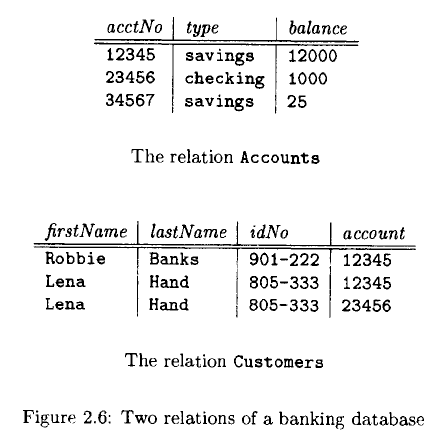
\includegraphics[width=0.6\linewidth]{images/worksheet_1_1.png}
    \end{center}

    \begin{enumerate}[a)]
        \item The attributes of each relation
        \item The tuples of each relation
        \item The components of one tuple from each relation
        \item The database schema
        \item A suitable domain for each attribute
        \item Another equivalent way to present each relation
    \end{enumerate}

    \item \textbf{Exercise 2.2.2:} In section 2.2.7 we suggested that there are many
    exmaples of attributes that are created for the purpose of serving as keys of
    relations. Give some additional examples.


    \item \textbf{Exericse 2.3.1} In this exercise we introduce one of our running
    examples of a relational database schema. The database schema consists of four relations,
    whose schemas are:

    \bigskip

    \begin{lstlisting}
    Product(maker, model, type)
    PC(model, speed, ram, hd, price)
    Laptop(model, speed, ram, hd, screen, price)
    Printer(model, color, type, price)
    \end{lstlisting}

    The \textbf{Product} relation gives the manufacturer, model number and type
    (PC< laptop, or printer) of various products. We assume for convenience that
    model numbers are unique over all manufactuers and product types; that assumption is
    not relaistic, and a real database would include a code for the manufacturer
    as part of the model number. The PC relation gives for each model number that
    is a PC the speed (of the processor, in gigahertz), the amount of RAM (in megabytes),
    the size of the hard disk (in gigabytes), and the price. The \textbf{Laptop}
    relation is similar, except that the screen size (in inches) is also included. The
    \textbf{Printer} relation records for each printer model wether the printer
    produces color output (true, if so), the process type (laser or ink-jet, typically),
    and the price.

    \bigskip

    Write the following declarations:

    \begin{enumerate}[a)]
        \item A suitable schema for relation \textbf{Product}
        \item A suitable schema for relation \textbf{Laptop}
        \item A suitable schema for relation \textbf{Printer}
        \item An alteration to your \textbf{Printer} schema from (d) to delete
        the attribute \textbf{color}
        \item An alternation to your \textbf{Laptop} schema from (c) to add the
        attribute \textbf{od} (optical-disk, e.g. cd or dvd). Let the default value
        for this attribute be `\textbf{none}' if the laptop does not have an optical
        disk.
    \end{enumerate}

    \item \textbf{Exericse 2.3.2} This exercise introduces another running example,
    concerning World War II capital ships. It involves the following relations:

    \bigskip

    \begin{lstlisting}
    Classes(class, type, country, numGuns, bore, displacement)
    Ships(name, class, launched)
    Battles(name, date)
    Outcomes(ship, battle, result)
    \end{lstlisting}

    \textbf{Ships} are bult in `classes' from the same design, and the class is
    usually named for the first ship of that class. The relation \textbf{Classes}
    records the name of the class, the type (`bb' for battleship or `bc' for battlecruiser),
    the country that built the ship, the number of main guns, the bore (diameter of
    the gun barrel, in inches) of the main guns, and the displacement (weight, in tones).
    Relation \textbf{Ships} records the name of the ship, the name of its class,
    and the year in which the ship was launched. Relation \textbf{Battles} gives
    the name and date battles involving these ships, and relation \textbf{Outcome}
    gives the result (sunk, damaged or ok) for each ship in each battle.

    \bigskip

    Write the following  declarations

    \bigskip

    \begin{enumerate}[a)]
        \item A suitable schema for relation \textbf{Classes}
        \item A suitable schema for relation \textbf{Ships}
        \item A suitable schema for relation \textbf{Battles}
        \item A suitable schema for relation \textbf{Outcomes}
        \item An alteration to your \textbf{Classes} relation from (a) to delete
        the attribute \textbf{bore}
        \item An alteration to your \textbf{Ships} relation from (b) to include
        attribute \textbf{yard} giving the shipard where the ship was built.
    \end{enumerate}
\end{enumerate}

\bigskip

\underline{\textbf{Reference}}

\bigskip

\begin{enumerate}[1)]
    \item Stanford: CS145 - Introduction to Databases, \href{http://infolab.stanford.edu/~ullman/fcdb/aut07/index.html}{link}
\end{enumerate}

\end{document}